\documentclass[12pt]{article}
\usepackage[T1]{fontenc} 
\usepackage[portuguese]{babel}
\usepackage{hyphenat}
% use se você precisar forçar a separação de sílabas em quebra de linha
\hyphenation{mate-mática recu-perar}
\usepackage{graphicx}
\graphicspath{images/}
\usepackage{csquotes}
\usepackage{subfiles}
\usepackage{amsmath}
\usepackage{csvsimple} 
\usepackage{geometry}
\geometry{
    a4paper,
    left=3cm,
    top = 3cm,
    right=2cm,
    bottom=2cm
}
\setlength{\parindent}{4em}
%\setlength{\parskip}{1em}
\renewcommand{\baselinestretch}{1.5}

\usepackage[dvipsnames]{xcolor}
\definecolor{alert}{RGB}{201, 58, 128}
\setlength {\marginparwidth }{2cm} 
\usepackage[colorinlistoftodos]{todonotes}
\usepackage{comment}
\usepackage{subcaption}
\DeclareUnicodeCharacter{0301}{*************************************}
\usepackage{enumitem}

\title{TÍTULO}
\author{autor}

\begin{document}

% CAPA
\thispagestyle{empty}

    
    \begin{flushright}
        \begin{huge}
            \textbf{RELATÓRIO}\\[3,5cm]
        \end{huge}
%% CSS: Podemos usar um título mais genérico agora e depois discutir um definitivo
{\bf \LARGE  TÍTULO}

\bigskip
        
        Leandro Zangirolami Trovões (Orientando)\\
        Carlos da Silva dos Santos (Orientador)\\
        Universidade Federal do ABC\\[5,5cm]
    \end{flushright}

    \vfill
    
    \begin{center}
        Santo André,\\
        Agosto de 2024
    \end{center}
    
    \newpage
\bigskip

\begin{center}
\noindent{\bf \Large Resumo}
\end{center}

\begin{quote}
[Contexto, visão geral do método, etc]
\end{quote}

\begin{center}
Santo André, julho de 2024
\end{center}

\newpage
\bigskip

\section{Introdução}
\label{sec:introducao}

\begin{comment}
doença sem cura, caracterizada pelo aumento de pressão intra-ocular que causa dados ao nervo ótico.
buscar fonte, WHO Nao explica direito
\end{comment}

%% CSS: usar o ~ antes do \cite impede que o latex quebre linha entre 
%       o texto e a anotação
Principal causa de cegueira irreversível no mundo~\cite{steinmetz_causes_2021}, o glaucoma é uma doença sem cura, caracterizada pelo dano progressivo ao nervo ótico~\cite{who_2019}. Estima-se que, em 2020, 3,6 milhões de pessoas com 50 anos ou mais já tenham perdido a visão para o Glaucoma~\cite{steinmetz_causes_2021} e um estudo de 2014 ainda projeta que 111.8 milhões de pessoas sejam afetadas pela doença no ano de 2040.~\cite{tham_global_2014}.

Assintomática em seus estágios iniciais, conforme avança, a doença causa perda de visão periférica e, se não for tratada, pode levar a perda total da visão. O tratamento pode retardar ou prevenir a progressão, mas depende de um diagnóstico precoce, geralmente antes mesmo dos primeiros sintomas~\cite{who_2019}.

\begin{comment}
O tratamento consiste em reduzir a pressão intra-ocular e 

fatores de risco: idade, histórico familiar

OMS: General population screening for glaucoma is not currently
considered to be cost-effective in most settings (63). Therefore,
routine eye examinations are recommended for high-risk individuals
as early detection is essential for the protection of visual function. 
\end{comment}

Uma das formas de identificar a doença é por meio da fundoscopia ou exame de fundo de olho, no qual é possível observar alterações características, muitas vezes antes mesmo que a perda de visão se torne detectável~\cite{weinreb_2016}. Um exemplo de imagem obtida nesse exame é apresentado na Figura~\ref{fig:fundus}.
\begin{comment}

Dentre as características observadas estão: 1, 2, 3, 4 e 5. cite{"Five rules to evaluate the optic disc and retinal nerve fiber layer for glaucoma"}

A capacidade da inteligência artificial em --- atrai seu uso na medicina. cite{alguem}

uso de IA com imagens médicas aumentou\\



fazer a avaliação manual gera divergência entre médicos, falta de padronização -> podemos fazer de forma automática
\end{comment}

\begin{comment}
da pra falar que médicas acreditam no potencial da IA
tem essa pesquisa aqui mas me parece muito restrita: só australia e nova zelancia e só com  trainees
...médicos acreditam que IA vai melhorar o trabalho deles... \cite{scheetz_survey_2021}
\end{comment}


Recentemente, diversas técnicas de aprendizagem profunda vem sendo aplicadas no diagnóstico de doenças com base em imagens de fundo de olho, inclusive para o glaucoma~\cite{li_review_2021}. Para possibilitar o desenvolvimento desses modelos, bancos de dados com imagens de fundo de olho classificadas por oftalmologistas foram criados e alguns deles disponibilizados publicamente.%% CSS: citar os bancos de dados aqui

\begin{figure}[htb]
 \centering
 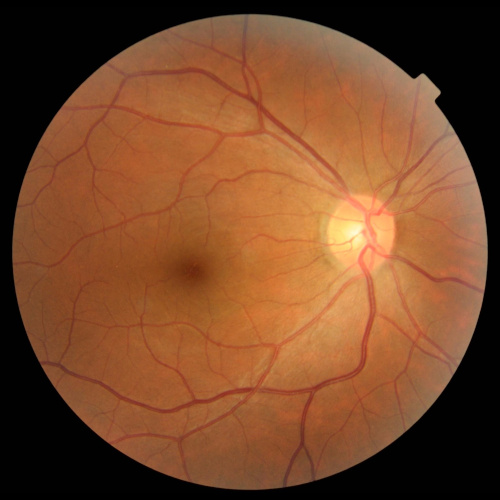
\includegraphics[width=0.3\textwidth]{images/TRAIN000004_cut.JPG}
 \caption{Imagem de fundo de olho. Obtida do banco de dados JustRAIGS.}
 \label{fig:fundus}
\end{figure}

% precisa se citação
A principal característica observada ao analisar o fundo de olho é a relação entre o tamanho da escavação em relação ao disco ótico, a primeira localizada ao centro do segundo, ambos destacados na Figura~\ref{fig:disk}. A razão entre o .. valor acima do normal é um indicativo do dano causado pela doença. 

\begin{figure}[htb]
 \centering
 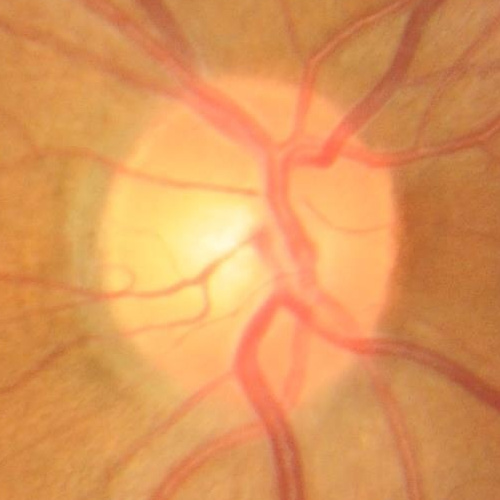
\includegraphics[width=0.3\textwidth]{images/disk.jpg}
 \caption{Disco ótico em destaque. Obtida do banco de dados JustRAIGS.}
 \label{fig:disk}
\end{figure}

% como encerrar?

Trabalhos relacionados conseguiram realizar a classificação de imagens entre glaucoma e não glaucoma utilizando diferentes técnicas 

O presente trabalho procura explorar...


\begin{comment}

usando redes neurais\\
e até mesmo técnicas de processamento de sinais\cite{Noronha2014}

porem:
\begin{itemize}
 \item datasets limitados (agora temos um de 100k imagens) e alguns são privados
 \item falta de justificativa, blackbox ~\cite{li_review_2021} 7.2.5, usar features adicionais para explicar decisão
\end{itemize}

suposições que precisam ser sustentadas:\\
1- razão OD e OC é a melhor forma de identificar glaucoma\\
2- CNN é melhor de que calcular a razão ente OD e OC: [Chen, 2015] afirma mas não sustenta. Cita [3]\\


2) Diaz-Pinto, 2019: usando CNN não precisa fazer segmentação perfeita do OD e do OC
"Important limitations of the methods that are based on handcrafted characteristics (CDR, Area Cup/Disc ratio (ACDR), vessel kinks and ISNT rule) is the significant disagreement in estimating them even between expert human graders. For that reason, new algorithms have been focused on automatic feature extraction such as the data-driven methods [3] and convolutional neural networks (CNNs)."\\
Menciona alguns trabalhos que foram pela abordagem da segmentação e os resultados obtidos.



investigar:
Chen, 2015: 17 5 6 14, 2, 12, 13\\
Noronha, 2014: 9, 16, 17, 18

\end{comment}


\begin{table}[htb]
    \centering
    \begin{tabular}{|c|c|c|}
    \hline
    Nome & Nº de imagens & Ano de publicação \\
    \hline
    REFUGE & 1200 & 2020 \\
    \hline
    DRISHTI-GS1 & 101 & 2015 \\
    \hline
    JustRAIGS & 101.442 & 2024 \\
    \hline
    \end{tabular}
    \caption{Bancos de dados para avaliação de glaucoma}
    \label{tab:datasets}
\end{table}


\begin{table}[htb]
    \centering
    \begin{tabular}{|l|l|l|l|c|c|}
    \hline
    Autores          & Método          & Imagens & Banco        & ACC     & AUC   \\
    \hline
    Chen, 2015       & CNN própria     &         & ORIGA        & -       & 0.831 \\
    \hline
    Chen, 2015       & CNN própria     &         & ORIGA + SCES & -       & 0.887 \\
    \hline
    Noronha, 2014    & Cumulantes      & 272     &              & 0.847  &  -     \\
    \hline
    Diaz-Pinto, 2019 & Xception        &         & -            &        &        \\
    \hline
    \end{tabular}
    \caption{Trabalhos anteriores e resultados obtidos}
    \label{tab:trabalhos}
\end{table}


\bigskip

O restante do texto é organizado da seguinte maneira: em primeiro lugar, apresentamos os objetivos deste trabalho na Seção~\ref{sec:objetivo}. Em seguida, a Seção~\ref{sec:revisao} 


\section{Objetivos}
\label{sec:objetivo}

segmentação da região de interesse

classificação 

\section{Plano de trabalho}
\label{sec:revisao}

\subsection{Fundamentos de Aprendizado de Máquina}
\label{sec:aprendizado}

\subsection{Métricas de Classificação}
\label{sec:metricas}


\section{Materiais e Métodos} 
\label{sec:metodos}


Escrevendo em \emph{itálico} ou \textbf{negrito}.

Uma lista de itens
\begin{itemize}
 \item Um
 \item Dois
\end{itemize}

Agora com numeração:
\begin{enumerate}
    \item Primeiro
    \item Segundo
\end{enumerate}

Agora com sequência alfabética:
\begin{enumerate}[label=(\alph*)]
    \item Primeiro
    \item Segundo
\end{enumerate}

Exemplo de expressão matemática em meio ao texto: $x \in [0, 1]$, outro exemplo: $f(x) = \frac{1}{1+e^{-x}}$.

Exemplo de equação numerada e como referenciar: veja a equação~(\ref{eq:somatoria}).
\begin{equation}
    \label{eq:somatoria}
    p(x) = \sum_{x=1}^{10} \frac{1}{x^2}
\end{equation}

Para incluir uma equação sem numeração, use o símbolo * (veja no arquivo .tex):
\begin{equation*}
    \label{eq:somatoria2}
    p(x) = \sum_{x=1}^{10} \frac{1}{\exp({x})}
\end{equation*}



\subsection{Conjuntos de dados}
\label{sec:dados}


\subsection{Recursos computacionais}
\label{sec:recursos}

Bibliotecas de software, infra-estrutura


\subsection{Resultados} 
\label{sec:resultados}


\begin{figure}[htb]
 \centering
 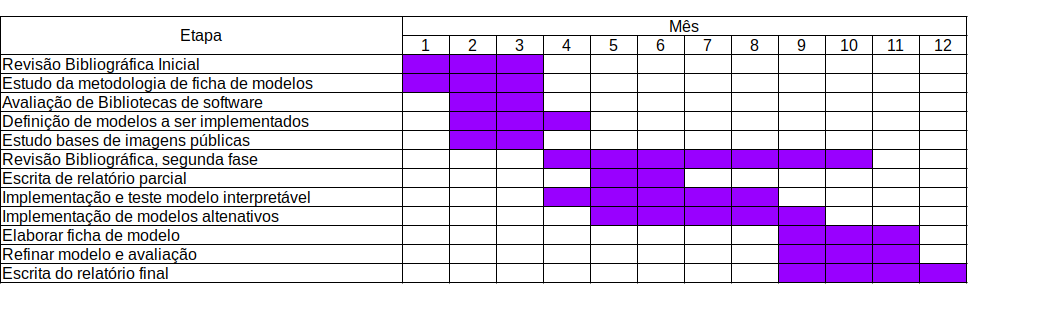
\includegraphics[width=1.0\textwidth]{images/crono2022}
 \caption{Cronograma de execução da proposta}
 \label{fig:crono}
\end{figure}


A Figura~\ref{fig:crono} apresenta o cronograma proposto...

\bibliographystyle{alpha}%{hapalike}
\bibliography{ref.bib}

\end{document}
